\chapter{Evaluation}\label{chapter:evaluation}

In the previous chapter(Chapter~\ref{chapter:methodology}), we detailed the entire workflow and underlying mechanisms of our proposed model. This chapter focuses on the evaluation of the results obtained throughout the study, providing an analysis of the model's performance and reasoning about the outcomes achieved.

Given that abnormal behavior detection is just one potential application of the developed model, the evaluation emphasizes its overall performance. Specifically, this chapter will compare results across different models applied to the same video, analyze the performance of the JODIE model on individual videos, evaluate the baseline results using Hidden Markov Models (HMM), and assess the impact of incorporating state embeddings into the JODIE framework.

Table~\ref{tab:dataset_statistic} and figure \ref{fig:dataset_statistic} offers an overview of the dataset used in the study. The dataset originates from experimental videos recorded with 15 participants, each contributing approximately two videos. The duration of each video ranges from 20 to 40 minutes, with each video containing around 13 to 16 nodes and 5000 to 15000 edges.

To further assess the model's scalability and generalization capabilities, we created a combined video by concatenating all the source videos. This combined dataset aims to test whether the model can predict driver behavior across all participants within a single learning process. The combined video has a total duration of approximately 10 hours, with 16 nodes and 287,644 edges. The number of nodes in the dataset shows only slight variation across videos. However, significant differences are observed in the number of edges and the video duration. As such, these latter factors—edge count and video duration—are considered the primary contributors to variations in model performance when applying the same model to different datasets.

Since our goal is to make predictions within dynamic graphs, it is essential to account for both \textbf{old nodes} that have appeared in previous time steps and \textbf{new nodes} that have not yet been observed. Both cases are integral to evaluating the model’s ability to generalize and adapt to evolving graph structures.

\clearpage


\begin{longtable}{lcccc}
        \toprule
    Participators        & Video    & \multicolumn{1}{l}{duration} & Number of Nodes& Number of Edges\\
        \midrule
    all                 & combined & 10:15:31                     & 16    &287644  \\
        \midrule
    \multirow{2}{*}{1}  & vp1\_1   & 00:21:10                     & 14    &8871     \\
                        & vp1\_2   & 00:23:49                     & 14    &8022          \\
        \midrule
    \multirow{2}{*}{2}  & vp2\_1   & 00:25:13                     & 15    &7291          \\
                        & vp2\_2   & 00:22:42                     & 14    &11865          \\
        \midrule
    \multirow{2}{*}{3}  & vp3\_1   & 00:22:22                     & 14    &9086          \\
                        & vp3\_2   & 00:18:11                     & 14    &6298          \\
        \midrule
    \multirow{2}{*}{4}  & vp4\_1   & 00:36:59                     & 15    &15497          \\
                        & vp4\_2   & 00:30:18                     & 15    &8626          \\
        \midrule
    \multirow{2}{*}{5}  & vp5\_1   & 00:29:37                     & 15    &13511          \\
                        & vp5\_2   & 00:21:39                     & 15    &7172          \\
        \midrule
    \multirow{2}{*}{6}  & vp6\_1   & 00:30:01                     & 16    &10056          \\
                        & vp6\_2   & 00:23:47                     & 15    &7878          \\
        \midrule
    \multirow{2}{*}{7}  & vp7\_1   & 00:23:07                     & 15    &9450          \\
                        & vp7\_2   & 00:15:28                     & 13    &5418          \\
        \midrule
    \multirow{2}{*}{8}  & vp8\_1   & 00:25:37                     & 15    &12513          \\
                        & vp8\_2   & 00:22:11                     & 14    &9748          \\
        \midrule
    9                   & vp9\_1   & 00:16:58                     & 14    &9057          \\
        \midrule
    \multirow{2}{*}{10} & vp10\_1  & 00:23:31                     & 15    &10524          \\
                        & vp10\_2  & 00:23:05                     & 13    &7534          \\
        \midrule
    \multirow{2}{*}{11} & vp11\_1  & 00:20:53                     & 11    &9157          \\
                        & vp11\_2  & 00:15:16                     & 13    &7193          \\
        \midrule
    \multirow{2}{*}{12} & vp12\_1  & 00:22:09                     & 16    &10451          \\
                        & vp12\_2  & 00:28:11                     & 15    &14807          \\
        \midrule
    \multirow{2}{*}{13} & vp13\_1  & 00:25:51                     & 13    &9518          \\
                        & vp13\_2  & 00:22:37                     & 14    &8319          \\
        \midrule
    \multirow{2}{*}{14} & vp14\_1  & 00:27:19                     & 14    &15539          \\
                        & vp14\_2  & 00:24:49                     & 13    &13889          \\
        \midrule
    \multirow{2}{*}{15} & vp15\_1  & 00:25:46                     & 14    &6873          \\
                        & vp15\_2  & 00:21:55                     & 13    &7621          \\
        \bottomrule

    \caption{The statistic of the dynamic graph derived from the source videos}
    \label{tab:dataset_statistic}
\end{longtable}

\clearpage
\begin{figure}[h]
    \centering
    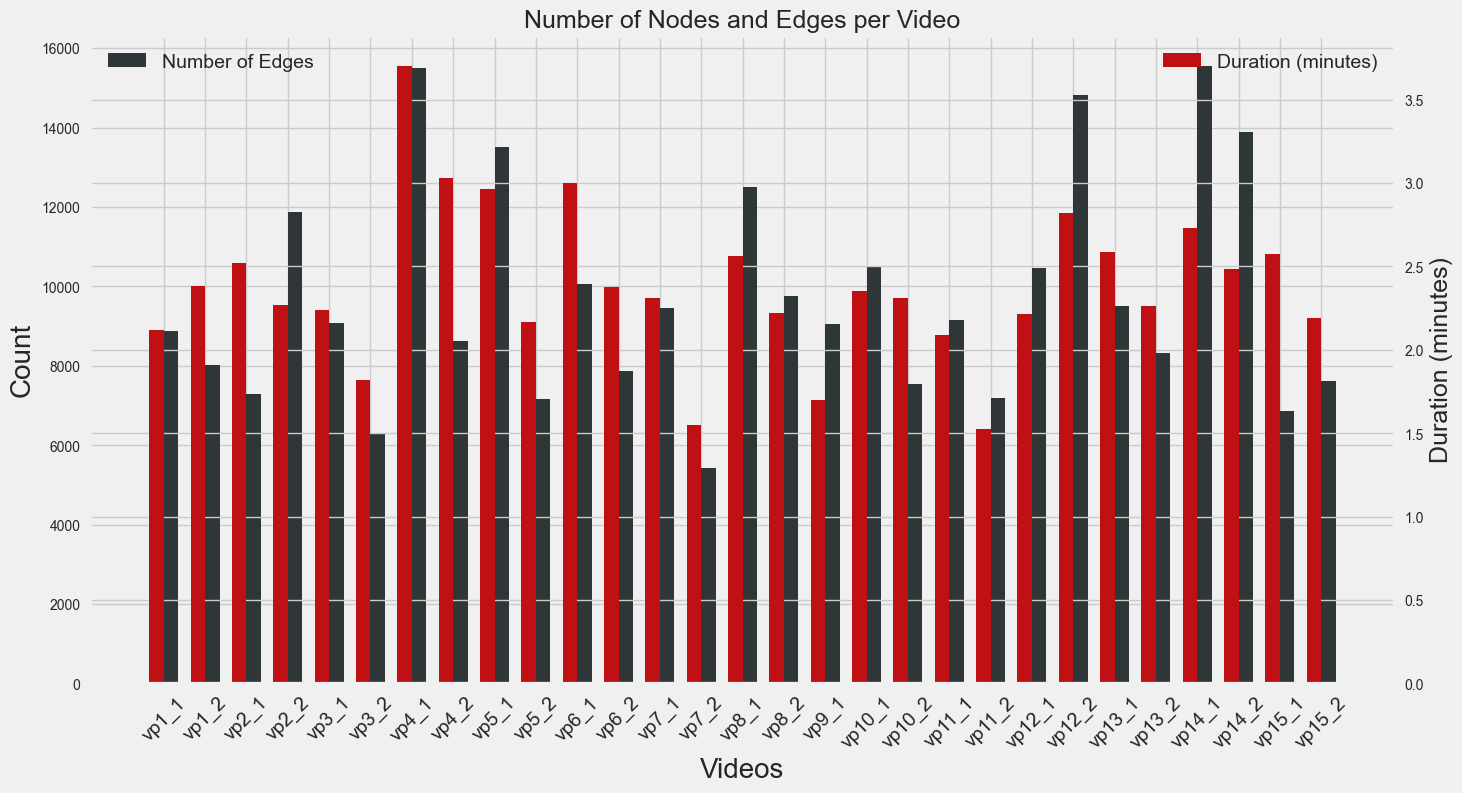
\includegraphics[width=\textwidth]{figures/05_data_statistic.png}
    \caption{Part of the statistic of the dataset}
    \label{fig:dataset_statistic}
\end{figure}

As for measurement, In our study, we utilize the \textbf{AU-ROC} and \textbf{AP} metric to evaluate and compare the performance of different models, as it provides a robust measure of a model's ability to distinguish between classes, particularly in imbalanced datasets. 

\textbf{AU-ROC (Area Under the Receiver Operating Characteristic Curve)} measures a model's classification ability by plotting the trade-off between the True Positive Rate (TPR) and False Positive Rate (FPR) across thresholds. It is calculated as: 

\[
\text{TPR} = \frac{\text{TP}}{\text{TP} + \text{FN}}, \quad \text{FPR} = \frac{\text{FP}}{\text{FP} + \text{TN}}
\]

An AU-ROC score of 1 indicates perfect classification, 0.5 implies random guessing, and values below 0.5 suggest poor performance. 
It is particularly effective for imbalanced datasets.

\textbf{Average Precision (AP)} measures a model's ability to balance precision and recall, summarizing the area under the Precision-Recall (PR) curve, here:
\begin{itemize}
    \item Precision = $\frac{\text{TP}}{\text{TP} + \text{FP}}$
    \item Recall = $\frac{\text{TP}}{\text{TP} + \text{FN}}$
\end{itemize}
It is particularly useful for imbalanced datasets, capturing the ranking quality of positive instances over negatives. AP is calculated as:

\[
\text{AP} = \sum_{i=1}^n \left( R_i - R_{i-1} \right) P_i
\]


where $P_i$ is precision and $R_i$ is recall at the $i^{th}$ threshold. An AP of 1.0 indicates perfect ranking, while 0.0 reflects completely incorrect predictions. It is widely used in tasks like object detection and retrieval.



\section{Model Performance Analysis}


The first step in the evaluation is a comparison of all models to identify the best-performing one in the basic task, which is to make a simple prediction on edge. Such task is achieved by training all the models with the video \textbf{vp01run1} and evaluating their performance using the AU-ROC metric. The whole training porcess is based on \textbf{DGB}\cite{poursafaei2022towards} The models considered in this comparison include \textbf{JODIE}, \textbf{TGN}, \textbf{DyRep}, and \textbf{CAW-N}.

The results are presented in Figure~\ref{fig:comparison} . Notably, the \textbf{CAW-N} model operates based on a random walking process, which limits its predictions to the existing graph. As a result, it does not produce separate outcomes for old and new node predictions.

As expected, the \textbf{JODIE} model demonstrates superior performance compared to the other three models, with \textbf{TGN} also delivering strong results. This aligns with the conclusions drawn in the previous chapter, reinforcing the robustness of these models.

Figure~\ref{fig:loss_comparison} provides clear evidence supporting our conclusions. The \textbf{JODIE} model demonstrates consistently strong performance with an optimal loss curve, indicating effective learning. The \textbf{TGN} model also performs well, though its final loss value is slightly higher than that of \textbf{JODIE}. In contrast, the \textbf{CAW-N} model exhibits signs of overfitting, as evidenced by its abrupt convergence to suboptimal solutions within very few epochs. Meanwhile, the \textbf{DyRep} model maintains a consistently high loss value throughout the training process, suggesting an inability to capture the underlying patterns in the dataset—indicative of underfitting.

\begin{figure}[h]
    \centering
    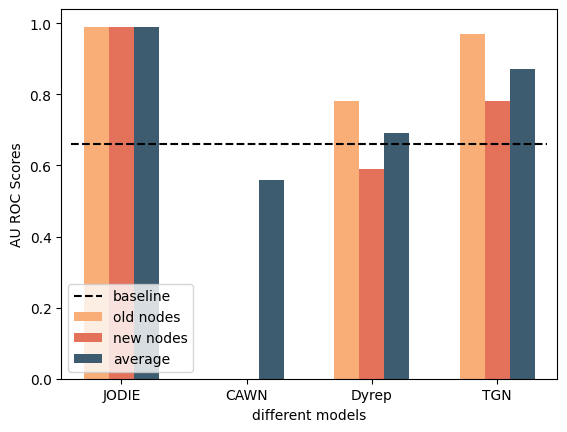
\includegraphics[width=0.6\textwidth]{figures/05_different_model_selection.png}
    \caption{The comparison between different models}
    \label{fig:comparison}
\end{figure}

\begin{figure}
    \centering
    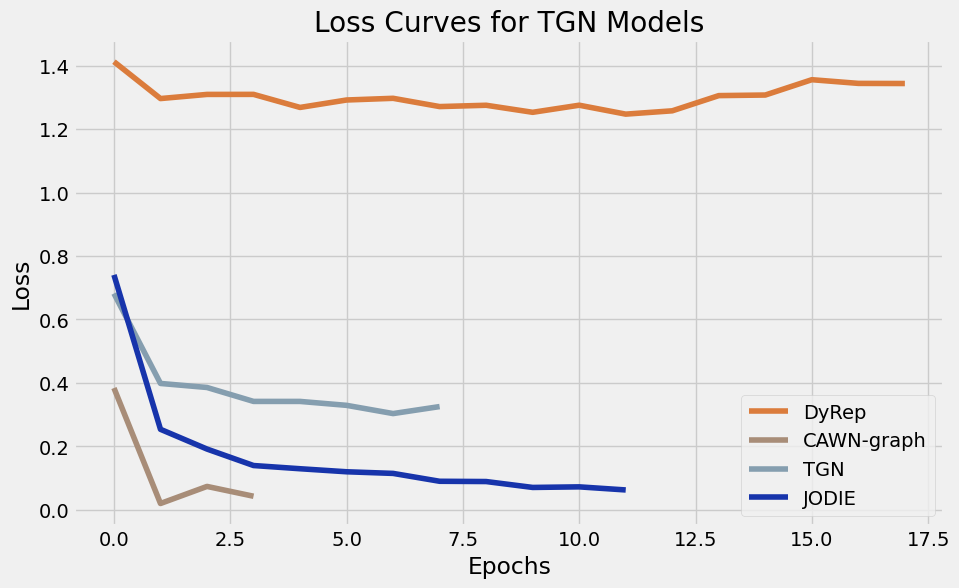
\includegraphics[width=0.8\textwidth]{figures/05_model_loss.png}
    \caption{training process between different models}
    \label{fig:loss_comparison}
\end{figure}
% the statistic of the dataset(timelenth)

\section{JODIE Results}


The decision to train the model with the original \textbf{JODIE} model serves two primary purposes. First, it allows us to validate our earlier hypothesis that JODIE exhibits superior performance across most videos in our dataset. Second, it provides a benchmark for comparison with the modified model incorporating state embeddings.

The evaluation of JODIE on individual videos demonstrates its robustness in predicting dynamic behavior, with results shown in Figure~\ref{fig:JODIE_results}. The model achieves consistent performance, with AU-ROC scores and APC approaching 1 across all original videos. This high accuracy can be attributed to the model's simplicity when edge states are excluded, relying only on single interactions per time period. Moreover, JODIE performs well in predicting both old and new nodes, indicating its ability to generalize across different node types.

However, challenges arise when training on the combined graph, which merges all videos. The increased complexity of this dataset—characterized by 15 participants, a significantly larger number of edges, and an extended duration—appears to hinder the model's performance. Despite this, JODIE remains the most effective model in our experiments when trained on graphs generated from individual videos in the dataset, further supporting its selection as a baseline.



\begin{figure}
    \centering
    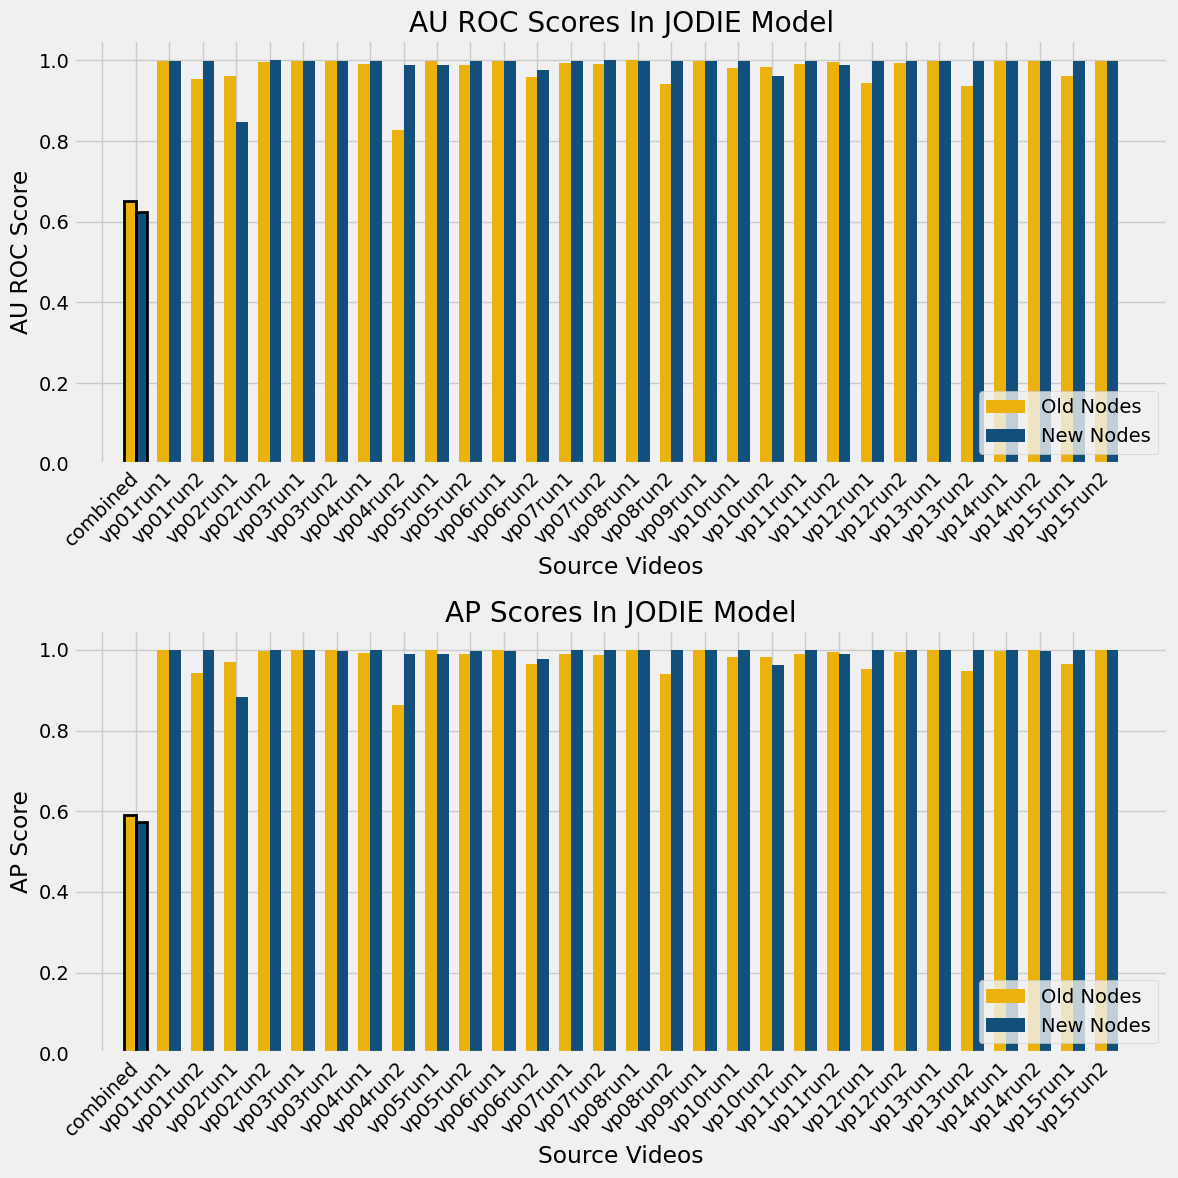
\includegraphics[width=\textwidth]{figures/05_JODIE.png}
    \caption{Dynamic Behavior Prediction Using JODIE}
    \label{fig:JODIE_results}
\end{figure}

\clearpage

\section{HMM Evaluation}



At this stage, the basic prediction tasks can already be performed on the dynamic graphs prepared for learning. However, none of the given models can predict both the edges and their corresponding states on the dynamic graphs effectively. To address this limitation, we first consider some classic models that offer the possiblity of future behavior prediction in some time-consequent datasets.

As is discussed before, we decide to evaluate the performance of Hidden Markov Models (HMM) on the same dataset. The HMM model is trained using the same dynamic graph structure as the JODIE model, with identical training and testing splits. The results are presented in Figure~\ref{fig:HMM_results}. Due to the inherent variability in the output of HMM, multiple training runs were conducted to provide a comprehensive understanding of its performance.

From the figure, it is evident that while HMM can learn from all the graphs and generate predictions for future behaviors, the results lack consistent patterns. In some cases, such as the training on \textit{vp03run1}, \textit{vp08run2}, \textit{vp10run2}, \textit{vp13run1}, and \textit{vp13run2}, peaks in the AU-ROC score are observed. However, these peaks are not replicable across different training runs on the same graphs, indicating that the HMM model lacks stability for dynamic graph prediction tasks. A similar inconsistency is also observed in the AP scores.

Although HMM offers a minimalist approach to the problem and demonstrates potential for application in dynamic graph prediction tasks, its inherent instability makes it unsuitable for real-world scenarios. The subsequent section presents our solution to this limitation by integrating state embeddings into the JODIE model.


\begin{figure}[h]
    \centering
    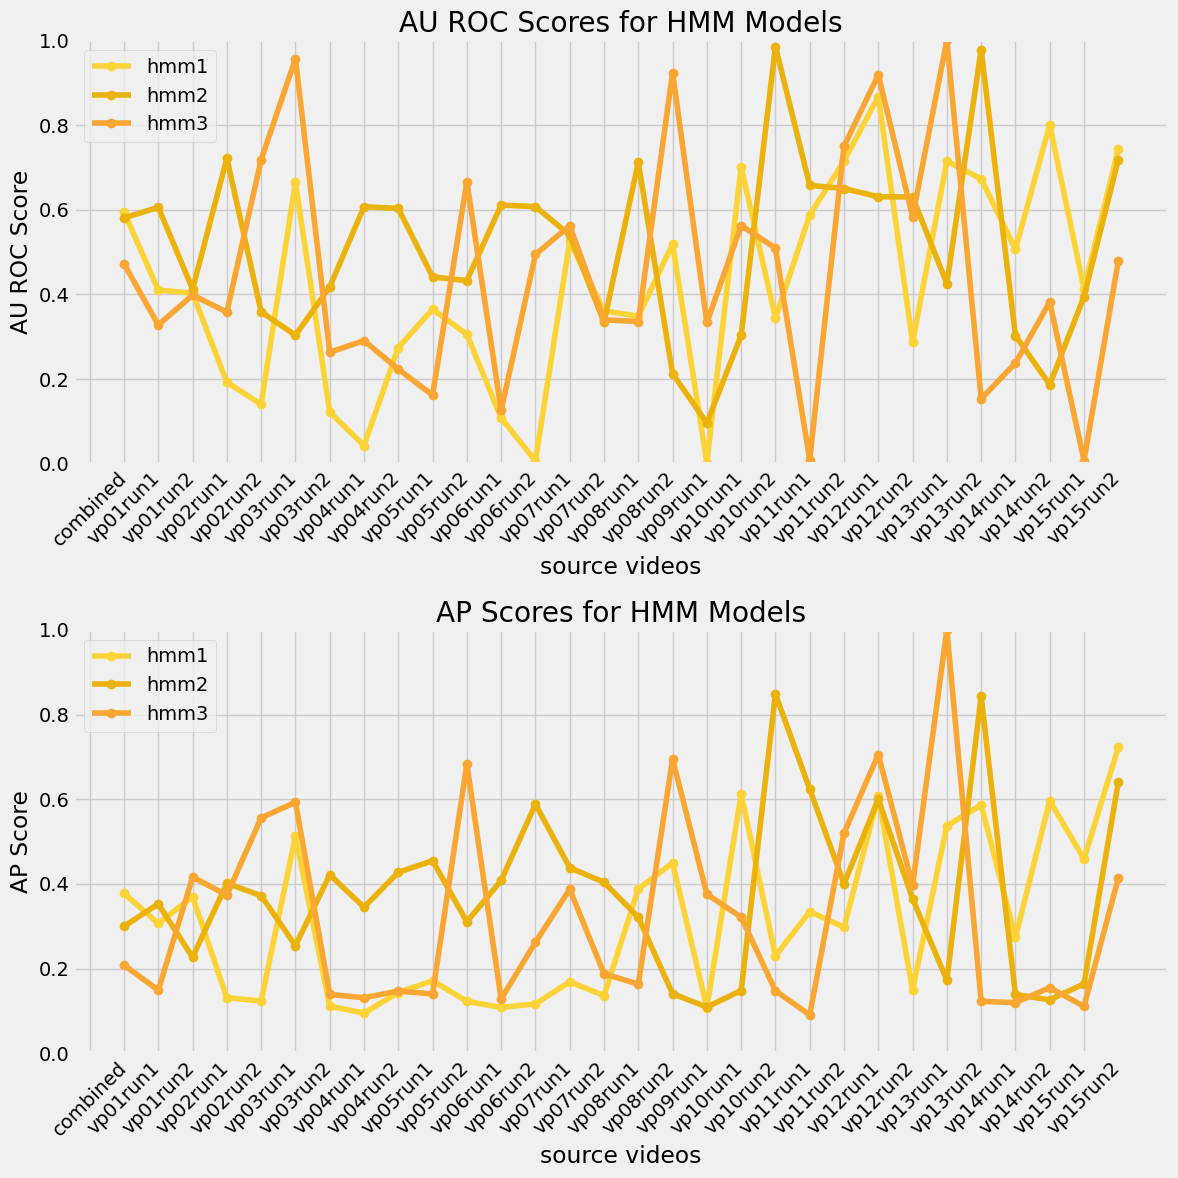
\includegraphics[width=\textwidth]{figures/05_baseline.png}
    \caption{Baseline Evaluation with Hidden Markov Models (HMM)}
    \label{fig:HMM_results}
\end{figure}


\clearpage
\section{Impact of State Embeddings}
Finally, we evaluate our proposed approach—JODIE with integrated state embeddings. The results, presented in Figure~\ref{fig:JODIE_state_embedding_results}, are derived from training the model on the same dataset as the original JODIE model, with the sole modification being the inclusion of state embeddings.
\begin{figure}[h]
    \centering
    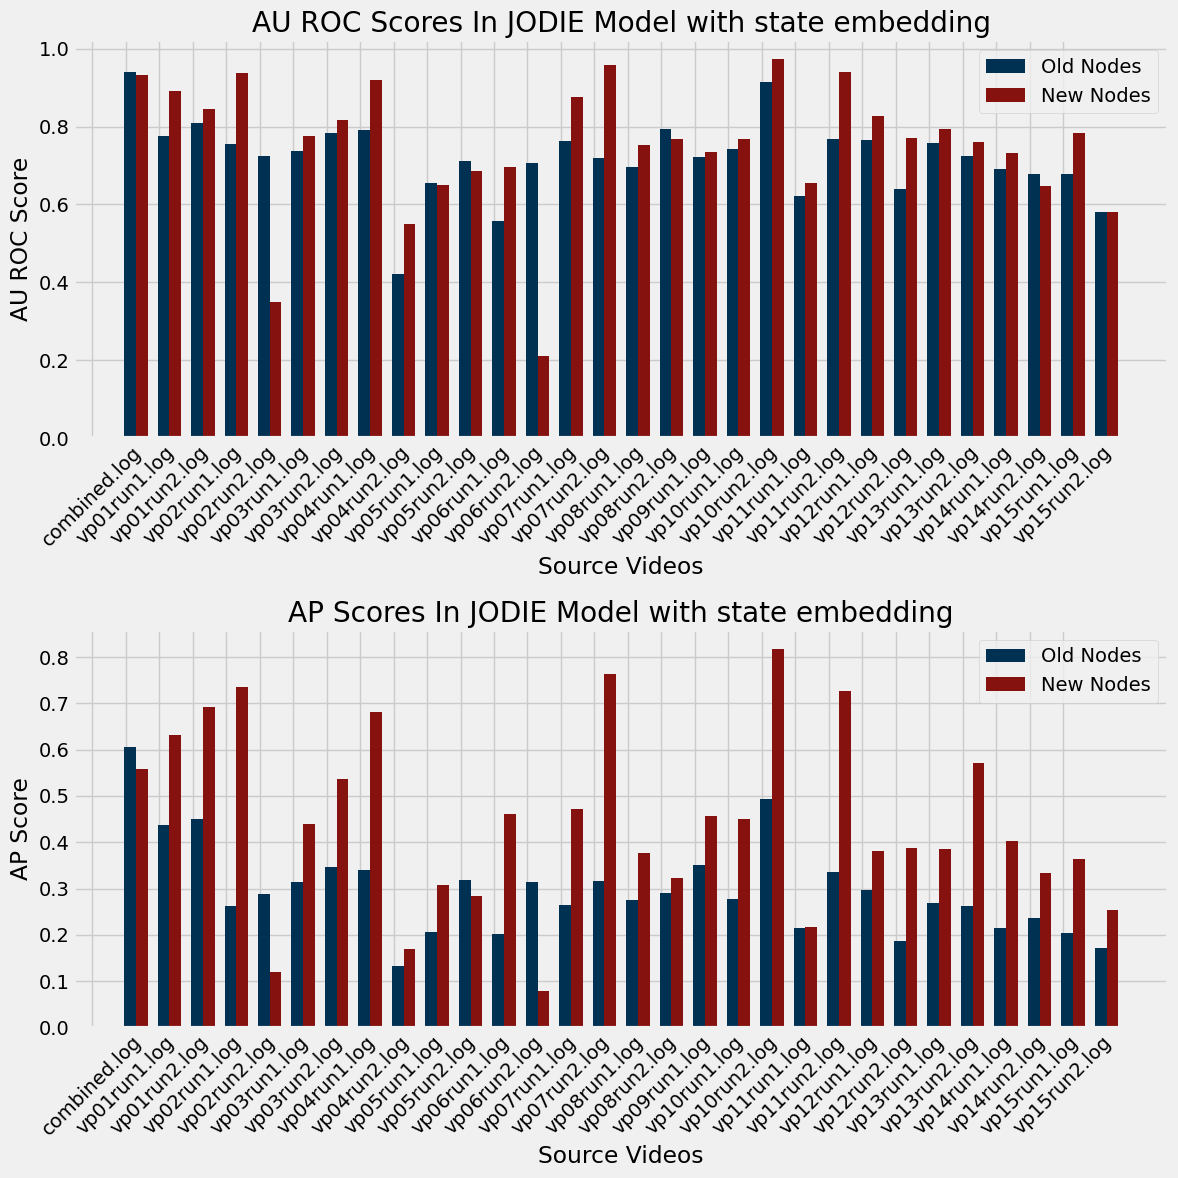
\includegraphics[width=\textwidth]{figures/05_JODIE_with_state.png}
    \caption{summery of JODIE with State Embedding}
    \label{fig:JODIE_state_embedding_results}
\end{figure}




The inclusion of state embeddings in the model unsurprisingly results in a drop in AUROC and AP scores. This can be attributed to the increased complexity of the model and the introduction of additional features. However, the model continues to perform well in dynamic graph prediction, as no significant failures are observed across prediction tasks. Interestingly, the combined graph, which aggregates data from multiple participants, achieves a higher AUROC score than several single-participant graphs. This provides strong evidence that the model is capable of generalizing predictions to larger datasets. Looking ahead, this suggests that incorporating more diverse models or larger datasets could further enhance its robustness. At the same time, it hints at possible underfitting in certain training runs, where the available dataset may not be sufficient for the model’s sophisticated structure. Encouragingly, this also highlights the model’s latent computational potential, which remains to be fully realized.

Another notable observation is the model’s superior performance in predicting new nodes compared to old ones. This aligns with the conclusion that state embeddings enhance the model’s sequential prediction capabilities. For our primary task of identifying potential driving risks, accurate prediction of new nodes is especially critical, as unexpected or previously unseen items often pose a greater hazard. Given that drivers tend to repeat their actions, the ability to reliably detect new nodes underscores the model’s importance and effectiveness in addressing safety-critical scenarios.



% TODO:discuss why AP is lower than AUROC, start from the definition of AP and AUROC


% TODO:yet still our work is much better than HMM

\begin{figure}[h]
    \centering
    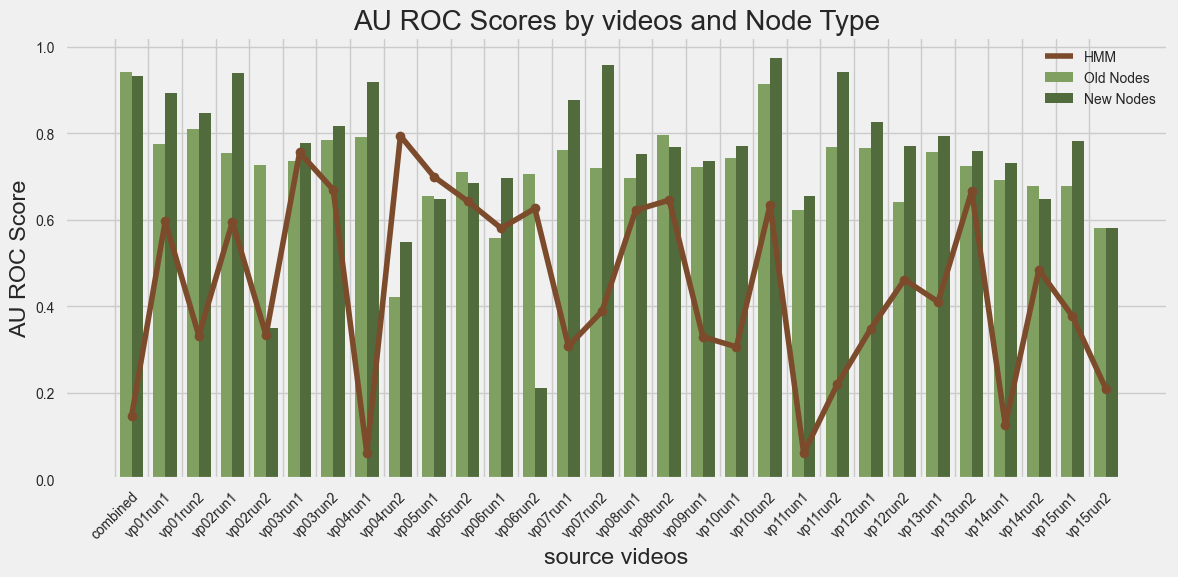
\includegraphics[width=\textwidth]{figures/05_JODIE_state_HMM_AUROC.png}
    \caption{summery of JODIE with State Embedding}
    \label{fig:JODIE_state_HMM_AUROC}
\end{figure}



\begin{figure}[h]
    \centering
    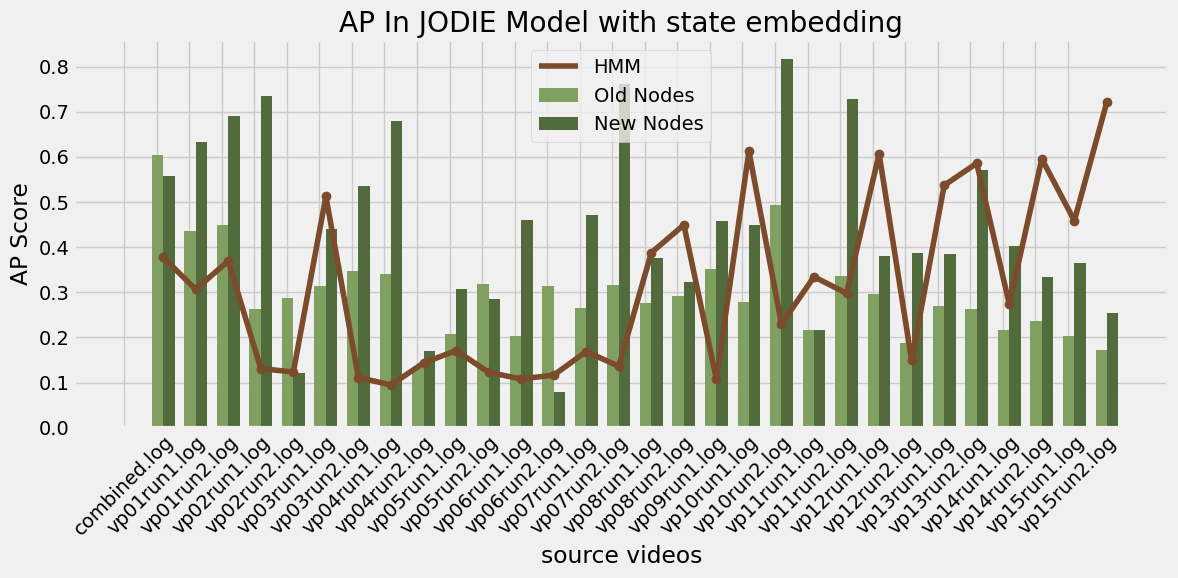
\includegraphics[width=\textwidth]{figures/05_JODIE_state_HMM_AP.png}
    \caption{summery of JODIE with State Embedding}
    \label{fig:JODIE_state_HMM_AP}
\end{figure}